%!TEX program = xelatex
\documentclass{article}
\usepackage[UTF8,scheme=plain]{ctex}

\usepackage{amsmath,amsthm,amsfonts,amssymb}
\usepackage{graphicx}
\usepackage{float}
\usepackage{subcaption}
\usepackage{booktabs,multirow,multicol}
\usepackage{indentfirst}
\usepackage{hyperref}
\usepackage{setspace}
\usepackage{listings}
\usepackage[ruled,noline]{algorithm2e}
\usepackage{bm}
\usepackage{xcolor}

\graphicspath{
    {./figure/}{./figures/}{./image/}{./images/}{./graphic/}{./graphics/}{./picture/}{./pictures/}
}


\title{NPDE~第2次实验报告}
\author{朱浩然 PB21000234}
\date{\today}

\begin{document}

\maketitle

\section{问题描述}
求下述偏微分方程初值问题在时刻$t=0.3$的近似解:
$$\left\{\begin{array}{ll}
    u_t=u_x,&-\infty<x<\infty,t>0,\\
    u(x,0)=sin(2\pi x),&-\infty<x<\infty,\\
    \text{周期性边界条件,且周期为:}1
\end{array}\right.$$

\section{方法}
该方程的精确解为$u(x,t)=sin(2\pi(x+t))$,对时空区域$[0,1]\times[0,1]$剖分(均分)如下:\par
时间:$t_{n}=n\cdot\Delta t, n=0,1,2,...,N,$时间步长$\Delta t=\frac{1}{N}$。\par
空间:$x_{j}=j\cdot\Delta x, j=0,1,2,...,J,$时间步长$\Delta x=\frac{1}{J}$。\par
定解条件:初始条件:$v_{j}^{0}=\sin(2\pi x_{j})$,边界条件:$v_{j}^{n}=v_{j+J}^{n}$。\par
记$v^n_j\approx u(x_{j},t_{n})$,时间导数用$u_{t} \approx \frac{u(x,t+\Delta t)-u(x,t)}{\Delta t}$近似,
空间导数分别用前差$u_{x} \approx \frac{u(x+\Delta x,t)-u(x,t)}{\Delta x}$和
中心差$u_{x} \approx \frac{u(x+\Delta x,t)-u(x-\Delta x,t)}{2\Delta x}$近似。\par
得到
$$\text{离散方程A}:v_j^{n+1}=v_j^n+\frac{\Delta t}{\Delta x}(v_{j+1}^n-v_j^n),$$
$$\text{离散方程B}:v_j^{n+1}=v_j^n+\frac{\Delta t}{2\Delta x}(v_{j+1}^n-v_{j-1}^n).$$
即分别为FTFS格式和FTCS格式的离散方程。\par
文件 HW2.cpp 使用c++编程计算,文件 HW2\underline{~}plot.m 使用MATLAB绘图。

\newpage
\section{结果}
问题1:取$\Delta x=0.02, \Delta t=0.01$,分别用离散方程A和离散方程B求上述偏微分方程初值问题在时刻$t=0.3$的近似解和精确解。\par
\begin{figure}[htbp]
    \centering
    \caption{问题1的解图像和误差图像}
    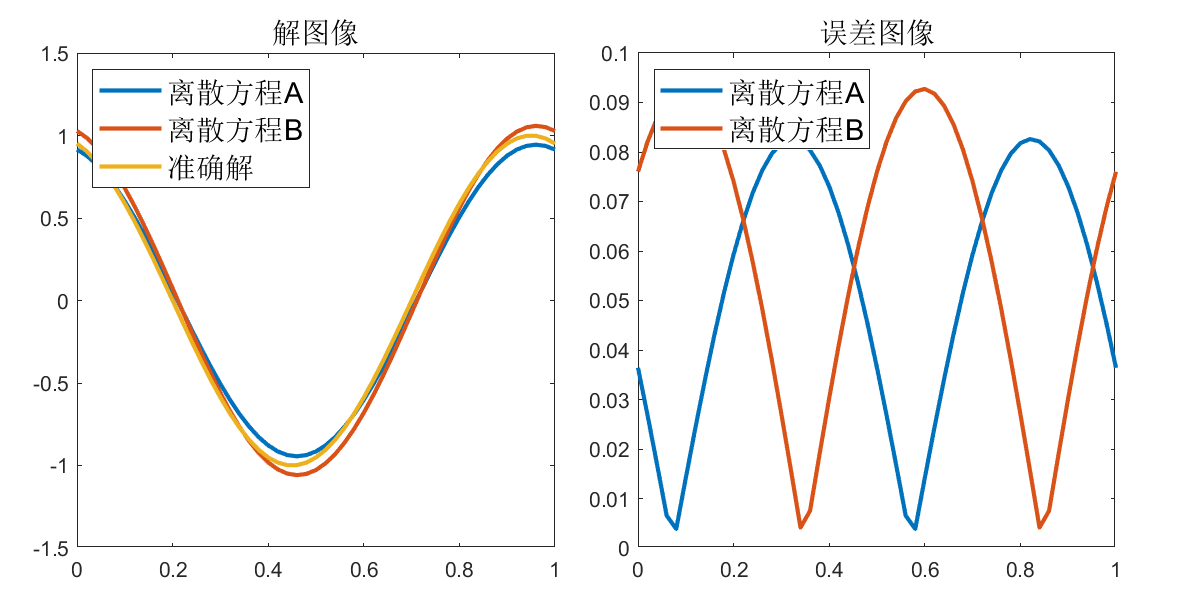
\includegraphics[width=\textwidth]{问题1.png}
\end{figure}
问题2:取$\Delta x=0.02, \Delta t=0.03$,分别用离散方程A和离散方程B求上述偏微分方程初值问题在时刻$t=0.3$的近似解和精确解。\par
\begin{figure}[htbp]
    \centering
    \caption{问题2的解图像和误差图像}
    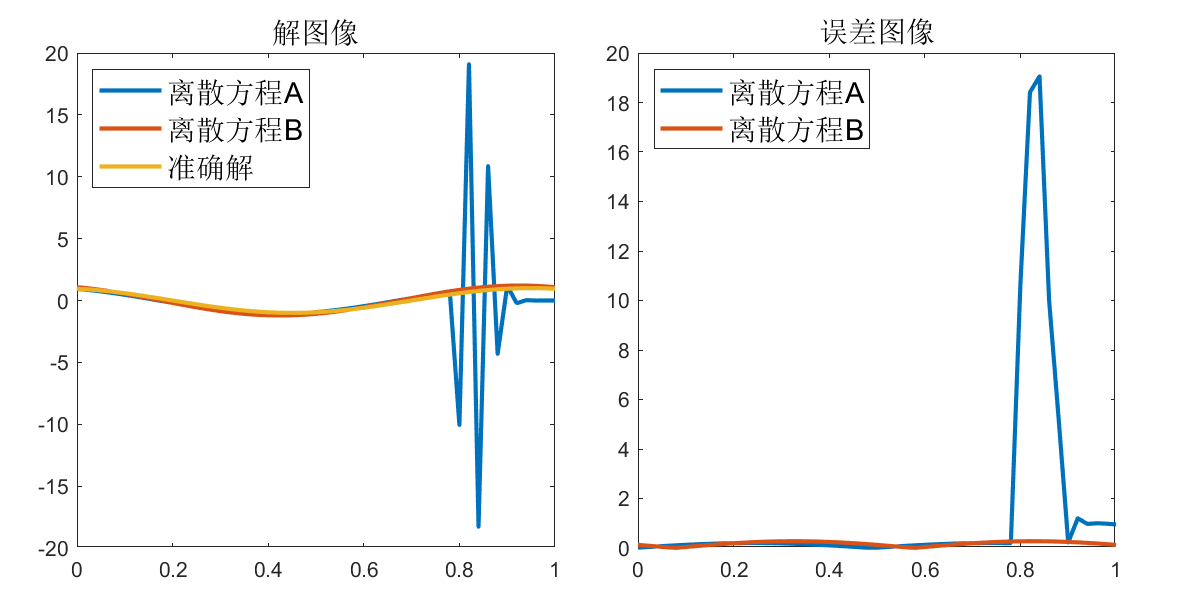
\includegraphics[width=\textwidth]{问题2.png}
\end{figure}

\section{总结}
FTCS格式比FTFS格式稳定,且dt/dx越大,FTFS格式越不稳定。

\end{document}
